\documentclass{article}

\usepackage{arxiv}

\usepackage[utf8]{inputenc} % allow utf-8 input
\usepackage[T1]{fontenc}    % use 8-bit T1 fonts
\usepackage{lmodern}        % https://github.com/rstudio/rticles/issues/343
\usepackage{hyperref}       % hyperlinks
\usepackage{url}            % simple URL typesetting
\usepackage{booktabs}       % professional-quality tables
\usepackage{amsfonts}       % blackboard math symbols
\usepackage{nicefrac}       % compact symbols for 1/2, etc.
\usepackage{microtype}      % microtypography
\usepackage{lipsum}
\usepackage{graphicx}

\title{A linear modelling exploration of goal scoring in the AFL}

\author{
    Trent Henderson
   \\
    OLET5608 \\
   \\
  \texttt{\href{mailto:then6675@uni.sydney.edu.au}{\nolinkurl{then6675@uni.sydney.edu.au}}} \\
  }


% Pandoc citation processing



\begin{document}
\maketitle

\def\tightlist{}


\begin{abstract}
Enter the text of your abstract here.
\end{abstract}


\setlength{\abovedisplayskip}{-15pt}
\setlength{\belowdisplayskip}{0pt}
\setlength{\abovedisplayshortskip}{0pt}
\setlength{\belowdisplayshortskip}{0pt}

\hypertarget{introduction}{%
\section{Introduction}\label{introduction}}

AFL is a highly popular Australian sports league that began in 1896 and
continues strongly today, with Grand Final match attendance (outside of
the anomalous COID-19-impacted 2020 season) approximating a sold out
100,000 each year at the traditional host venue - the Melbourne Cricket
Ground. An AFL match is won based on points, which can be accumulated by
kicking either a goal (worth six points) or a behind (worth one point).
Given the relative importance of goals-to-behinds and the rapid rise of
advanced analytics in sport, many, if not all, AFL teams are interested
in how they can score more goals.

Moreover, this pursuit of knowledge extends far past teams and players.
Websites such as FiveThirtyEight and Advanced Sports Analytics have
created a reliable source of insight and interactive analysis that only
continue to rise in popularity and sophistication. However, this form of
innovative and detailed sports analytics has yet to fully breach
Australian sports. While the AFL has dedicated talk show analysis
television programs such as AFL 360, The Front Bar, and Talking Footy,
these programs focus mostly on qualitative breakdowns of high-level
match statistics and not on statistical rigour. This report aims to
bridge some of this gap by providing a preliminary statistical
investigation of goal scoring in the AFL.

\hypertarget{the-importance-of-kicking-goals}{%
\subsection{The importance of kicking
goals}\label{the-importance-of-kicking-goals}}

As described above, goals are worth six points in AFL, meaning most
offensive activity is conducted so as to increase the likelihood and
number of goals that are scored. Their contribution to the probability
of a team winning a match is substantial, as highlighted by
\textbf{FIGURE 1} below, where a match outcome of 1 = win and 0 = loss.
The plot visualises the outputs of a logistic regression where the
number of goals scored by a team for a given match was used as a
predictor of binary match outcome (win versus loss). The number of goals
scored was statistically significant, such that for every one unit
increase in goals scored by a team, the odds of winning the match
increase by 1.07 (\emph{p} \textless.001, 95\% confidence interval =
1.07-1.08). The case for a team focusing their efforts on scoring more
goals is evident.

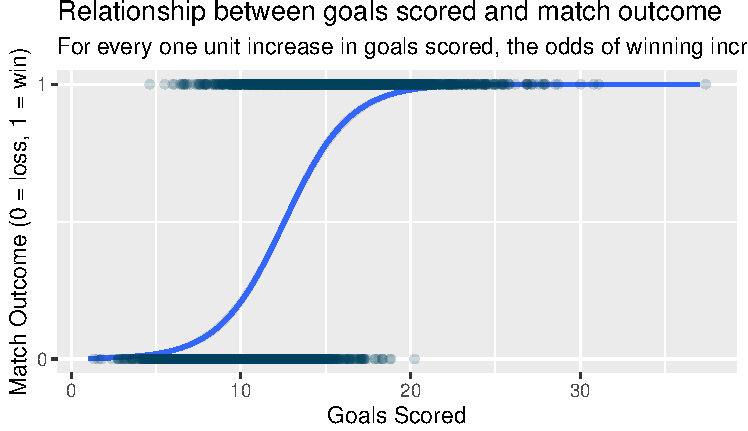
\includegraphics{OLET5608_TrentHenderson_files/figure-latex/unnamed-chunk-2-1.pdf}

However, as is the case with most high-level sport, winning games is not
as simple as \emph{just} kicking more goals. There are sometimes long
sequences of free-form and contested play that precede a goal being
kicked that can be hard to directly influence through coaching
interventions based off the notion of \emph{as a team we need to kick
more goals}. Instead, understanding the correlates and predictors of
goal scoring using a data-driven approach may reveal subtle nuances in
gameplay which could be used to tailor training and coaching approaches.
At an even more granular level, differences in how these different
gameplay attributes manifest for specific teams may lead to different
recommendations.

Specifically, this report aims to explore the following research
question: \emph{Which gameplay attributes are predictors of the number
of goals scored by teams in AFL matches?}

\hypertarget{data-set}{%
\section{Data set}\label{data-set}}

Historical AFL data has been made readily-accessible in an open-source
setting through the R package \texttt{fitzRoy} (see Day, Nguyen, and
Lane 2020). The package provides a simple API that accesses and
integrates a range of data sources that collate AFL data. Examples of
these sources include:

\begin{itemize}
  \item{AFL}
  \item{AFL Tables}
  \item{Squiggle}
  \item{FootyWire}
\end{itemize}

The data itself is diverse, covering domains as broad as player and
match statistics, Brownlow medal votes, betting odds, attendance
numbers, and match times. This report focuses on player and match
statistics by aggregating quantities of interest to team-per-match-level
sums using data for the 2010-2019 seasons, inclusive. This time period
is partially arbitrary, but was made on the basis of recency and
potential homogeneity. The 2020 season is a strong counter example of
this, where the season length was truncated and played almost entirely
in Queensland due to the impacts of COVID-19 This means the standard set
up of games - having a home and away team - was not normal in 2020 and
thus data for the entire season may represent a heterogenous set.

A small subset of variables were retained from the broader dataset. The
subset was developed based on the author's subject matter expertise of
the sport of AFL, with additional consideration given to not wanting to
specify an overly complex model. The variables retained were selected
based on their likely relationship to a team's goal scoring and whether
a team could change their gameplay to better target these predictors.
For example, the variable \emph{free kicks against} was not included, as
the number of free kicks given away by a team is not a core contributor
to the same team scoring goals.

The variables that were retained for the purposes of this analysis
included team-match-level counts of goals, marks, handballs, hit outs,
tackles, rebounds, inside 50s, clearances, clangers, free kicks for,
contested possessions, contested marks, and marks inside 50.

\hypertarget{analysis}{%
\section{Analysis}\label{analysis}}

A rigorous and detailed linear modelling pipeline was implemented. This
involved the following steps:

\begin{enumerate}
\def\labelenumi{\arabic{enumi}.}
\tightlist
\item
  Exploratory data analysis and preprocessing
\item
  Model fitting
\item
  Model assumption testing
\item
  Model re-specification (if required)
\item
  Model interpretation
\item
  Preliminary advanced model exploration
\end{enumerate}

\hypertarget{exploratory-data-analysis-and-visualisation}{%
\subsection{Exploratory data analysis and
visualisation}\label{exploratory-data-analysis-and-visualisation}}

Prior to modelling, the data were explored visually and numerically to
understand the empirical structure. \textbf{FIGURE X} below shows the
distributions of each quantitative variable.

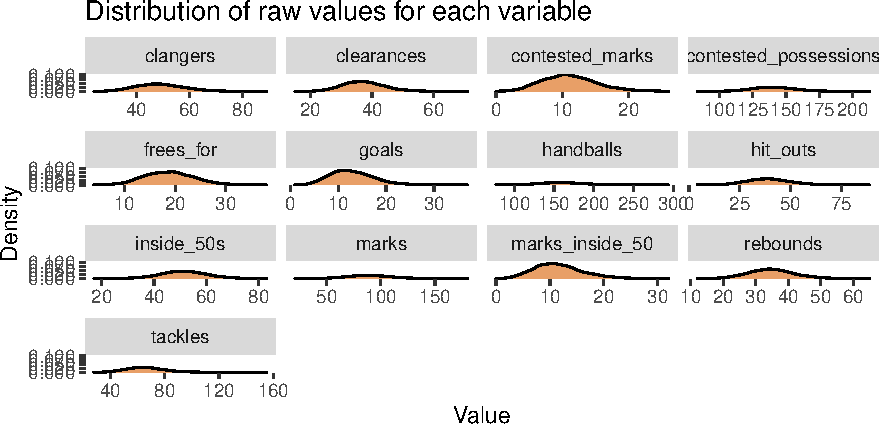
\includegraphics{OLET5608_TrentHenderson_files/figure-latex/unnamed-chunk-4-1.pdf}

The data were further explored using high-level summary statistics.
These are presented below in \textbf{FIGURE XX}. Note the large
difference in scales between the variables. To avoid issues with
high-variance predictors influencing linear modelling or producing
extremely low coefficients, all predictors were mean-centred and
standardised (z-scored) prior to modelling.

\% latex table generated in R 4.0.2 by xtable 1.8-4 package \% Mon May 3
23:12:36 2021

\begin{table}[ht]
\centering
\begin{tabular}{rl}
  \hline
 & type \\ 
  \hline
1 & numeric \\ 
   \hline
\end{tabular}
\end{table}

\hypertarget{model-fitting}{%
\subsection{Model fitting}\label{model-fitting}}

\hypertarget{model-assumption-testing}{%
\subsection{Model assumption testing}\label{model-assumption-testing}}

There are four core assumptions of linear regression model (see Faraway
2004). These include:

\begin{enumerate}
\def\labelenumi{\arabic{enumi}.}
\tightlist
\item
  Linear relationship between \texttt{X} and \texttt{y}
\item
  Independent observations
\item
  Homogeneity of variance
\item
  Normality of residuals
\end{enumerate}

Since it is known that the data used for this report as independent
observations, the following sections will focus on reporting the testing
of the other assumptions.

\hypertarget{assumption-1-linear-relationship}{%
\subsubsection{Assumption 1: Linear
relationship}\label{assumption-1-linear-relationship}}

The purpose of a linear model is to understand the relationship between
some number of predictors and a quantitative response variable. As such,
a linear model at its core assumes that all predictors are related
linearly to the response variable.

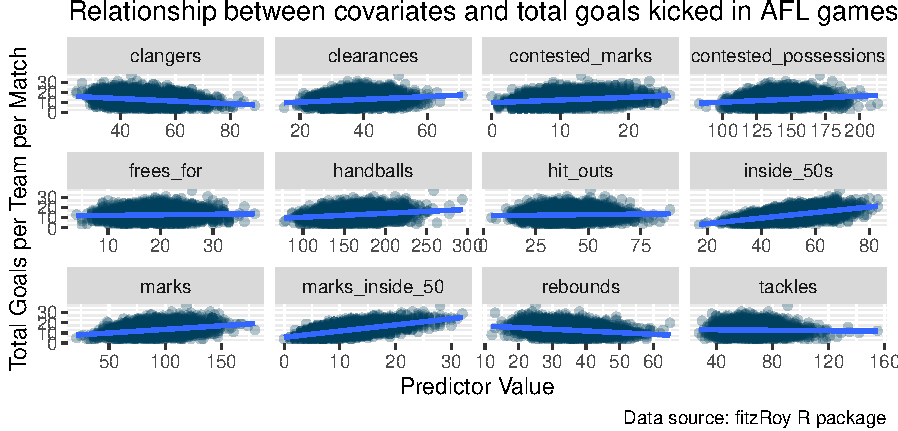
\includegraphics{OLET5608_TrentHenderson_files/figure-latex/unnamed-chunk-7-1.pdf}

A secondary visual test was conducted with a robust regression (using
M-estimation) as the plots above appeared to contain some potential
leverage points or outliers. The robust version of the plot is depicted
below in \textbf{FIGURE X}. With almost no visual difference between the
standard linear and the robust lienar approaches, the standard linear
model was taken forward.

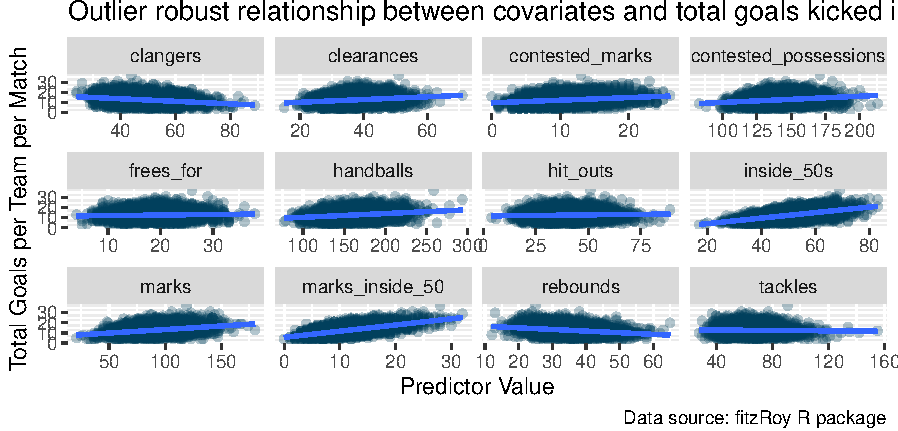
\includegraphics{OLET5608_TrentHenderson_files/figure-latex/unnamed-chunk-8-1.pdf}

While all variables were still being tested for appropriateness, a
variance inflation factor (VIF) test was undertaken to estimate
potential multicollinearity between the predictors. Multicollinearity is
an issue as it can drive imprecise estimates, change parameter value
signs, and impact \(R^2\). Different threshold values exist for the VIF,
with cutoffs ranging from values less than four being acceptable (see
Hair et al. 2010) to values less than ten being acceptable (see Hair et
al. 1995). Outputs from the VIF test are presented below. Evidently, no
predictor violates even the lowest bound commonly cited in the
literature, indicating no issue with multicollinearity.

\begin{verbatim}
##                Variables Tolerance      VIF
## 1                  marks 0.5689153 1.757731
## 2              handballs 0.8070175 1.239130
## 3               hit_outs 0.7752018 1.289987
## 4                tackles 0.7890447 1.267355
## 5               rebounds 0.7090882 1.410262
## 6             inside_50s 0.4915640 2.034323
## 7             clearances 0.5586642 1.789984
## 8               clangers 0.7929755 1.261073
## 9              frees_for 0.9170373 1.090468
## 10 contested_possessions 0.3844856 2.600878
## 11       contested_marks 0.7361132 1.358487
## 12       marks_inside_50 0.5647187 1.770793
\end{verbatim}

\hypertarget{assumption-2-homogeneity-of-variance}{%
\subsubsection{Assumption 2: Homogeneity of
variance}\label{assumption-2-homogeneity-of-variance}}

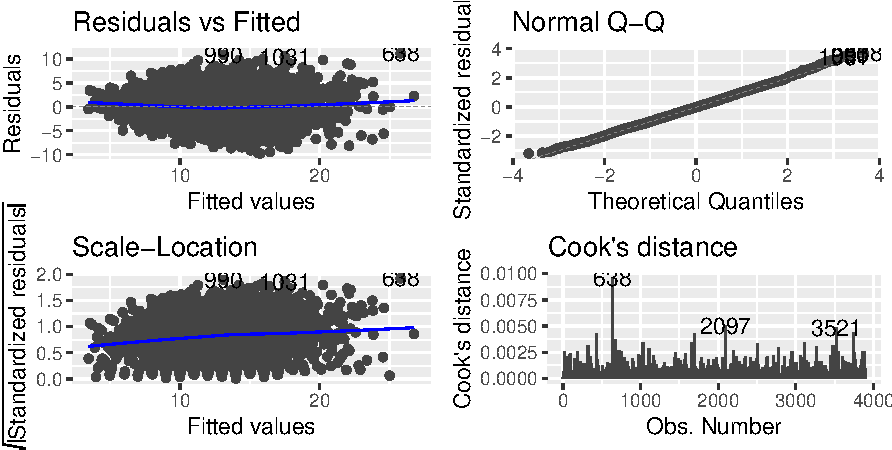
\includegraphics{OLET5608_TrentHenderson_files/figure-latex/unnamed-chunk-10-1.pdf}

\hypertarget{assumption-3-normality-of-residuals}{%
\subsubsection{Assumption 3: Normality of
residuals}\label{assumption-3-normality-of-residuals}}

\hypertarget{preliminary-advanced-model-exploration}{%
\subsection{Preliminary advanced model
exploration}\label{preliminary-advanced-model-exploration}}

One other model was fit in addition to the standard linear model - a
generalised additive model (GAM) (see Hastie and Tibshirani 1986). GAMs
further generalise the commonly-used generalised linear model (GLM) to
accommodate immensely powerful flexibility and potential to model
non-linearities. GAMs achieve this through the use of splines and basis
functions whose number is specified by a knot parameter, and who are
connected by polynomials. GAMs essentially enable the fitting of wiggly
functions over the data. The basic form of a GAM can be written as
follows, where the predictors are still entered linearly, but they are
instead modelled using some unknown smooth functions:

\[
y_i = \beta_0 + f_1(x_i) + f_2(x_i)... + f_n(x_n) + \epsilon_i
\]

Where \(\epsilon\) is (in the standard linear modelling case) Gaussian
noise \(\mathcal{N}(\mu,\sigma^2)\), specified by its mean and standard
deviation. Of course, similar to GLMs, this Gaussian noise assumption is
generalised to other probability distributions, though these are not the
considered in this report. The GAM for this report was fit in \texttt{R}
using the \texttt{mgcv} package (see Wood 2011). It was fit using
Restricted Maximum Likelihood for reduced-rank model parameter
estimation, as per advice by Wood (see Wood, n.d.).

\hypertarget{model-assumption-testing-1}{%
\subsubsection{Model assumption
testing}\label{model-assumption-testing-1}}

Similar to the standard linear model, core assumptions still need to
hold for the GAM. These were also tested, with a summary output
presented below in \textbf{FIGURE 1} generated by the \texttt{R} package
\texttt{mgcViz} (see Fasiolo et al. 2018).

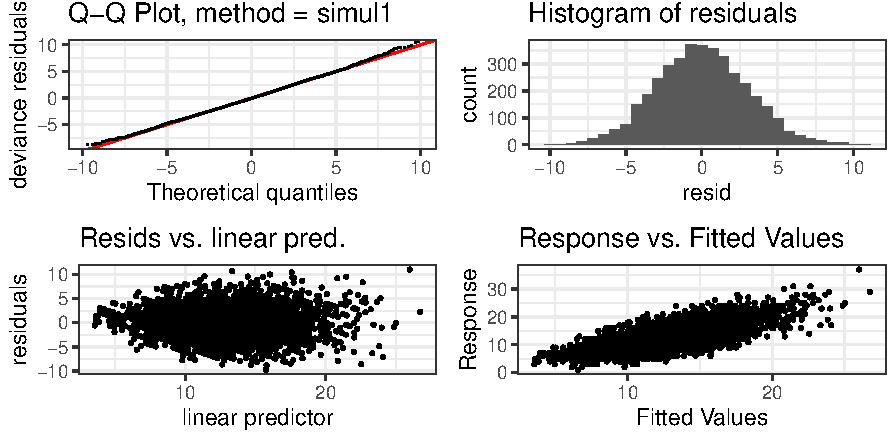
\includegraphics{OLET5608_TrentHenderson_files/figure-latex/unnamed-chunk-11-1.pdf}

\hypertarget{results}{%
\section{Results}\label{results}}

\hypertarget{linear-model}{%
\subsection{Linear model}\label{linear-model}}

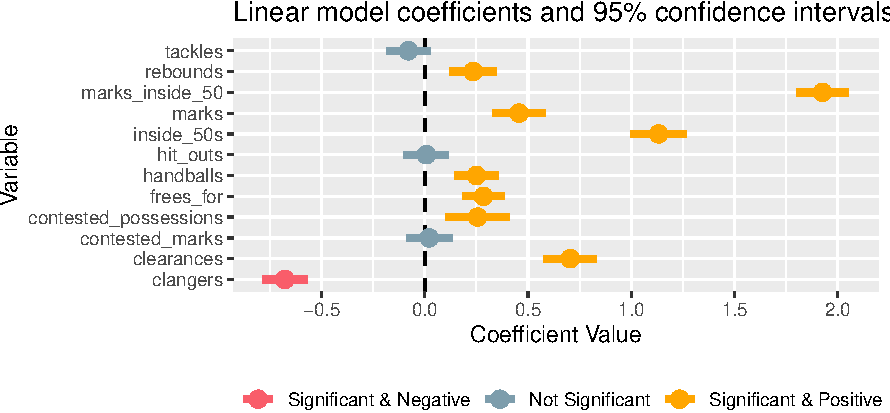
\includegraphics{OLET5608_TrentHenderson_files/figure-latex/unnamed-chunk-12-1.pdf}

A numerical exploration of coefficients is presented below. This table
also contains information regarding the overall model fit and
\emph{F}-statistic. The overall model is statistically significant,
\emph{F} = 370.77 (\emph{df} = 12; 3879), and explains approximately
53.4\% of the observed variance in goals scored.

\begin{table}[!htbp] \centering 
  \caption{} 
  \label{} 
\begin{tabular}{@{\extracolsep{5pt}}lc} 
\\[-1.8ex]\hline 
\hline \\[-1.8ex] 
 & \multicolumn{1}{c}{\textit{Dependent variable:}} \\ 
\cline{2-2} 
\\[-1.8ex] & goals \\ 
\hline \\[-1.8ex] 
 marks & 0.457$^{***}$ \\ 
  & (0.065) \\ 
  & \\ 
 handballs & 0.250$^{***}$ \\ 
  & (0.054) \\ 
  & \\ 
 hit\_outs & 0.008 \\ 
  & (0.055) \\ 
  & \\ 
 tackles & $-$0.079 \\ 
  & (0.055) \\ 
  & \\ 
 rebounds & 0.235$^{***}$ \\ 
  & (0.058) \\ 
  & \\ 
 inside\_50s & 1.133$^{***}$ \\ 
  & (0.070) \\ 
  & \\ 
 clearances & 0.705$^{***}$ \\ 
  & (0.065) \\ 
  & \\ 
 clangers & $-$0.677$^{***}$ \\ 
  & (0.055) \\ 
  & \\ 
 frees\_for & 0.284$^{***}$ \\ 
  & (0.051) \\ 
  & \\ 
 contested\_possessions & 0.256$^{***}$ \\ 
  & (0.079) \\ 
  & \\ 
 contested\_marks & 0.022 \\ 
  & (0.057) \\ 
  & \\ 
 marks\_inside\_50 & 1.926$^{***}$ \\ 
  & (0.065) \\ 
  & \\ 
 Constant & 12.812$^{***}$ \\ 
  & (0.049) \\ 
  & \\ 
\hline \\[-1.8ex] 
Observations & 3,892 \\ 
R$^{2}$ & 0.534 \\ 
Adjusted R$^{2}$ & 0.533 \\ 
Residual Std. Error & 3.044 (df = 3879) \\ 
F Statistic & 370.774$^{***}$ (df = 12; 3879) \\ 
\hline 
\hline \\[-1.8ex] 
\textit{Note:}  & \multicolumn{1}{r}{$^{*}$p$<$0.1; $^{**}$p$<$0.05; $^{***}$p$<$0.01} \\ 
\end{tabular} 
\end{table}

\hypertarget{gam}{%
\subsection{GAM}\label{gam}}

XX

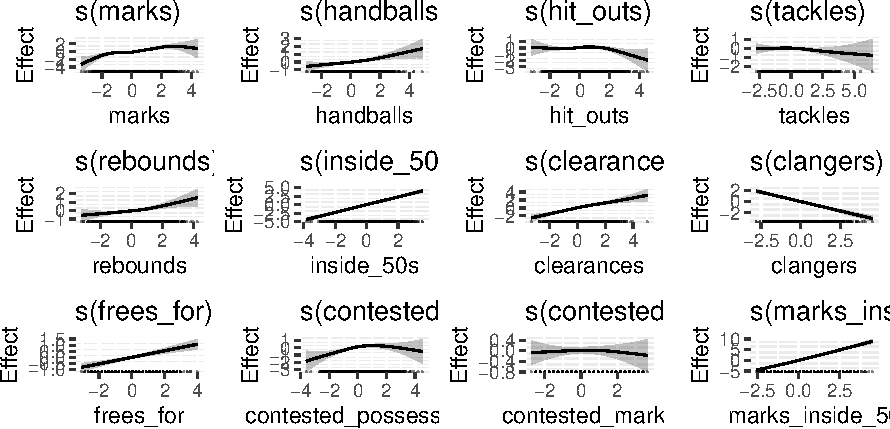
\includegraphics{OLET5608_TrentHenderson_files/figure-latex/gam-smooths-1.pdf}

\hypertarget{discussion}{%
\section{Discussion}\label{discussion}}

\hypertarget{references}{%
\section*{References}\label{references}}
\addcontentsline{toc}{section}{References}

\hypertarget{refs}{}
\leavevmode\hypertarget{ref-fitzRoy}{}%
Day, James, Robert Nguyen, and Oscar Lane. 2020. \emph{FitzRoy: Easily
Scrape and Process Afl Data}.
\url{https://CRAN.R-project.org/package=fitzRoy}.

\leavevmode\hypertarget{ref-R:Faraway:2004}{}%
Faraway, Julian J. 2004. \emph{Linear Models with R}. Chapman \&
Hall/CRC. \url{http://www.maths.bath.ac.uk/\%20jjf23/LMR/}.

\leavevmode\hypertarget{ref-mgcViz}{}%
Fasiolo, Matteo, Raphael Nedellec, Yannig Goude, and Simon N. Wood.
2018. ``Scalable Visualisation Methods for Modern Generalized Additive
Models.'' \emph{Arxiv Preprint}. \url{https://arxiv.org/abs/1707.03307}.

\leavevmode\hypertarget{ref-multi2}{}%
Hair, J. F., R. E. Anderson, R. L. Tatham, and W. C. Black. 1995.
\emph{Multivariate Data Analysis (3rd Ed.)}. Macmillan Publishing
Company, New York.

\leavevmode\hypertarget{ref-multi1}{}%
Hair, J. F., W. C. Black, B. J. Babin, and R. E. Anderson. 2010.
\emph{Multivariate Data Analysis (7th Ed.)}. Upper saddle River, New
Jersey: Pearson Education International.

\leavevmode\hypertarget{ref-10.1214ux2fssux2f1177013604}{}%
Hastie, Trevor, and Robert Tibshirani. 1986. ``Generalized Additive
Models.'' \emph{Statistical Science} 1 (3): 297--310.
\url{https://doi.org/10.1214/ss/1177013604}.

\leavevmode\hypertarget{ref-mgcv}{}%
Wood, S. N. 2011. ``Fast Stable Restricted Maximum Likelihood and
Marginal Likelihood Estimation of Semiparametric Generalized Linear
Models.'' \emph{Journal of the Royal Statistical Society (B)} 73 (1):
3--36.

\leavevmode\hypertarget{ref-wood}{}%
---------. n.d. ``Frequently Asked Questions for Package Mgcv.''
\url{http://web.mit.edu/~r/current/arch/i386_linux26/lib/R/library/mgcv/html/mgcv-FAQ.html}.

\bibliographystyle{unsrt}
\bibliography{references.bib}


\end{document}
